% Generated from shared citation records and relations.tikz
\documentclass[border=12pt]{standalone}
\def\pgfsysdriver{pgfsys-dvisvgm.def}
\usepackage[dvisvgm]{xcolor}
\usepackage{xeCJK}
\setCJKmainfont{HaranoAjiGothic-Regular.otf}[BoldFont=HaranoAjiGothic-Bold.otf]
\setCJKsansfont{HaranoAjiGothic-Regular.otf}[BoldFont=HaranoAjiGothic-Bold.otf]
\usepackage{amsmath,amssymb,tikz,lmodern}
\usetikzlibrary{arrows.meta,positioning,calc,fit,backgrounds}
\renewcommand{\familydefault}{\sfdefault}
\definecolor{ink}{HTML}{25322F}
\definecolor{green}{HTML}{246657}
\definecolor{tint}{HTML}{EEF4F0}
\definecolor{soft}{HTML}{C6D2CC}
\definecolor{muted}{HTML}{52615B}
\newif\ifJapanese
\newcommand{\Tx}[2]{\ifJapanese #1\else #2\fi}
\newcommand{\Eff}{\overline{\operatorname{Eff}}}
\newcommand{\heading}[3]{{\color{green}\bfseries #1\quad\Tx{#2}{#3}}\\[5pt]}
% A white rectangle makes the complete citation label clickable, including spaces.
\newcommand{\refurl}[2]{\special{dvisvgm:raw <a xlink:href="#1" target="_blank" rel="noopener noreferrer">}{\setlength{\fboxsep}{0pt}\colorbox{white}{\color{green}\underline{\strut #2}}}\special{dvisvgm:raw </a>}}

\tikzset{
 card/.style={draw=soft,fill=white,rounded corners=2pt,align=left,text=ink,font=\fontsize{10.5}{14}\selectfont,inner xsep=10pt,inner ysep=9pt,text width=13.2cm,minimum height=1.55cm},
 result/.style={card,draw=green,fill=tint,line width=.9pt},
 small/.style={card,text width=5.5cm},
 reason/.style={align=left,text=muted,font=\fontsize{9}{12}\selectfont,inner sep=0pt,text width=12cm},
 edge/.style={-{Stealth[length=2.4mm]},draw=green,line width=1pt},
}
\def\flow#1#2#3;{
 \coordinate (#2-from) at ($(#1.south)+(-6.2,0)$);
 \coordinate (#2-to) at ($(#2.north)+(-6.2,0)$);
 \draw[edge] (#2-from)--(#2-to);
 \node[reason,anchor=west] at ($(#2-from)!.5!(#2-to)+(.5,0)$) {#3};
}
% Shared style adapted from Schnell / Geometry Paper Digest; MIT attribution retained.

% Generated from citations.json; do not edit.
\newcommand{\Cite}[1]{\csname cite-#1\endcsname}
\expandafter\def\csname cite-catalog-source\endcsname{\shortstack[l]{\refurl{https://github.com/openai/math/blob/1581d4cbdd69a0faf34b2089614fe2a814316a6a/overview.pdf}{[OpenAICatalog, Catalogue 356, p. 38]}}}
\expandafter\def\csname cite-main\endcsname{\shortstack[l]{\refurl{https://github.com/openai/math/blob/1581d4cbdd69a0faf34b2089614fe2a814316a6a/preprints/Giglis-distributional-curvature-characterization-of-Alexandrov-spaces-September-24-2026/main.pdf}{[OpenAI26a, Theorem 1.1, p. 2]}}}
\expandafter\def\csname cite-forward\endcsname{\shortstack[l]{\refurl{https://github.com/openai/math/blob/1581d4cbdd69a0faf34b2089614fe2a814316a6a/preprints/Giglis-distributional-curvature-characterization-of-Alexandrov-spaces-September-24-2026/main.pdf}{[OpenAI26a, Theorem 3.1, p. 9]}}}
\expandafter\def\csname cite-index\endcsname{\shortstack[l]{\refurl{https://github.com/openai/math/blob/1581d4cbdd69a0faf34b2089614fe2a814316a6a/preprints/Giglis-distributional-curvature-characterization-of-Alexandrov-spaces-September-24-2026/main.pdf}{[OpenAI26a, Theorem 4.1, p. 24]}}}
\expandafter\def\csname cite-hessian\endcsname{\shortstack[l]{\refurl{https://github.com/openai/math/blob/1581d4cbdd69a0faf34b2089614fe2a814316a6a/preprints/Giglis-distributional-curvature-characterization-of-Alexandrov-spaces-September-24-2026/main.pdf}{[OpenAI26a, Theorem 5.10, pp. 46–47]}}}
\expandafter\def\csname cite-modification\endcsname{\shortstack[l]{\refurl{https://github.com/openai/math/blob/1581d4cbdd69a0faf34b2089614fe2a814316a6a/preprints/Giglis-distributional-curvature-characterization-of-Alexandrov-spaces-September-24-2026/main.pdf}{[OpenAI26a, Lemma 6.2, pp. 48–49]}}}
\expandafter\def\csname cite-interface\endcsname{\shortstack[l]{\refurl{https://github.com/openai/math/blob/1581d4cbdd69a0faf34b2089614fe2a814316a6a/preprints/Giglis-distributional-curvature-characterization-of-Alexandrov-spaces-September-24-2026/main.pdf}{[OpenAI26a, Theorem 6.1, p. 48]}}}
\expandafter\def\csname cite-comparison\endcsname{\shortstack[l]{\refurl{https://github.com/openai/math/blob/1581d4cbdd69a0faf34b2089614fe2a814316a6a/preprints/Giglis-distributional-curvature-characterization-of-Alexandrov-spaces-September-24-2026/main.pdf}{[OpenAI26a, Theorem 6.3, pp. 49–50]}}}
\expandafter\def\csname cite-companion\endcsname{\shortstack[l]{\refurl{https://github.com/openai/math/blob/1581d4cbdd69a0faf34b2089614fe2a814316a6a/preprints/Weak-Hessian-bounds-along-every-geodesic-in-RCD-spaces-September-24-2026/weak-hessian-geodesics.pdf}{[OpenAI26b, Theorem 1.1, p. 2]}}}

\Japanesefalse
\begin{document}
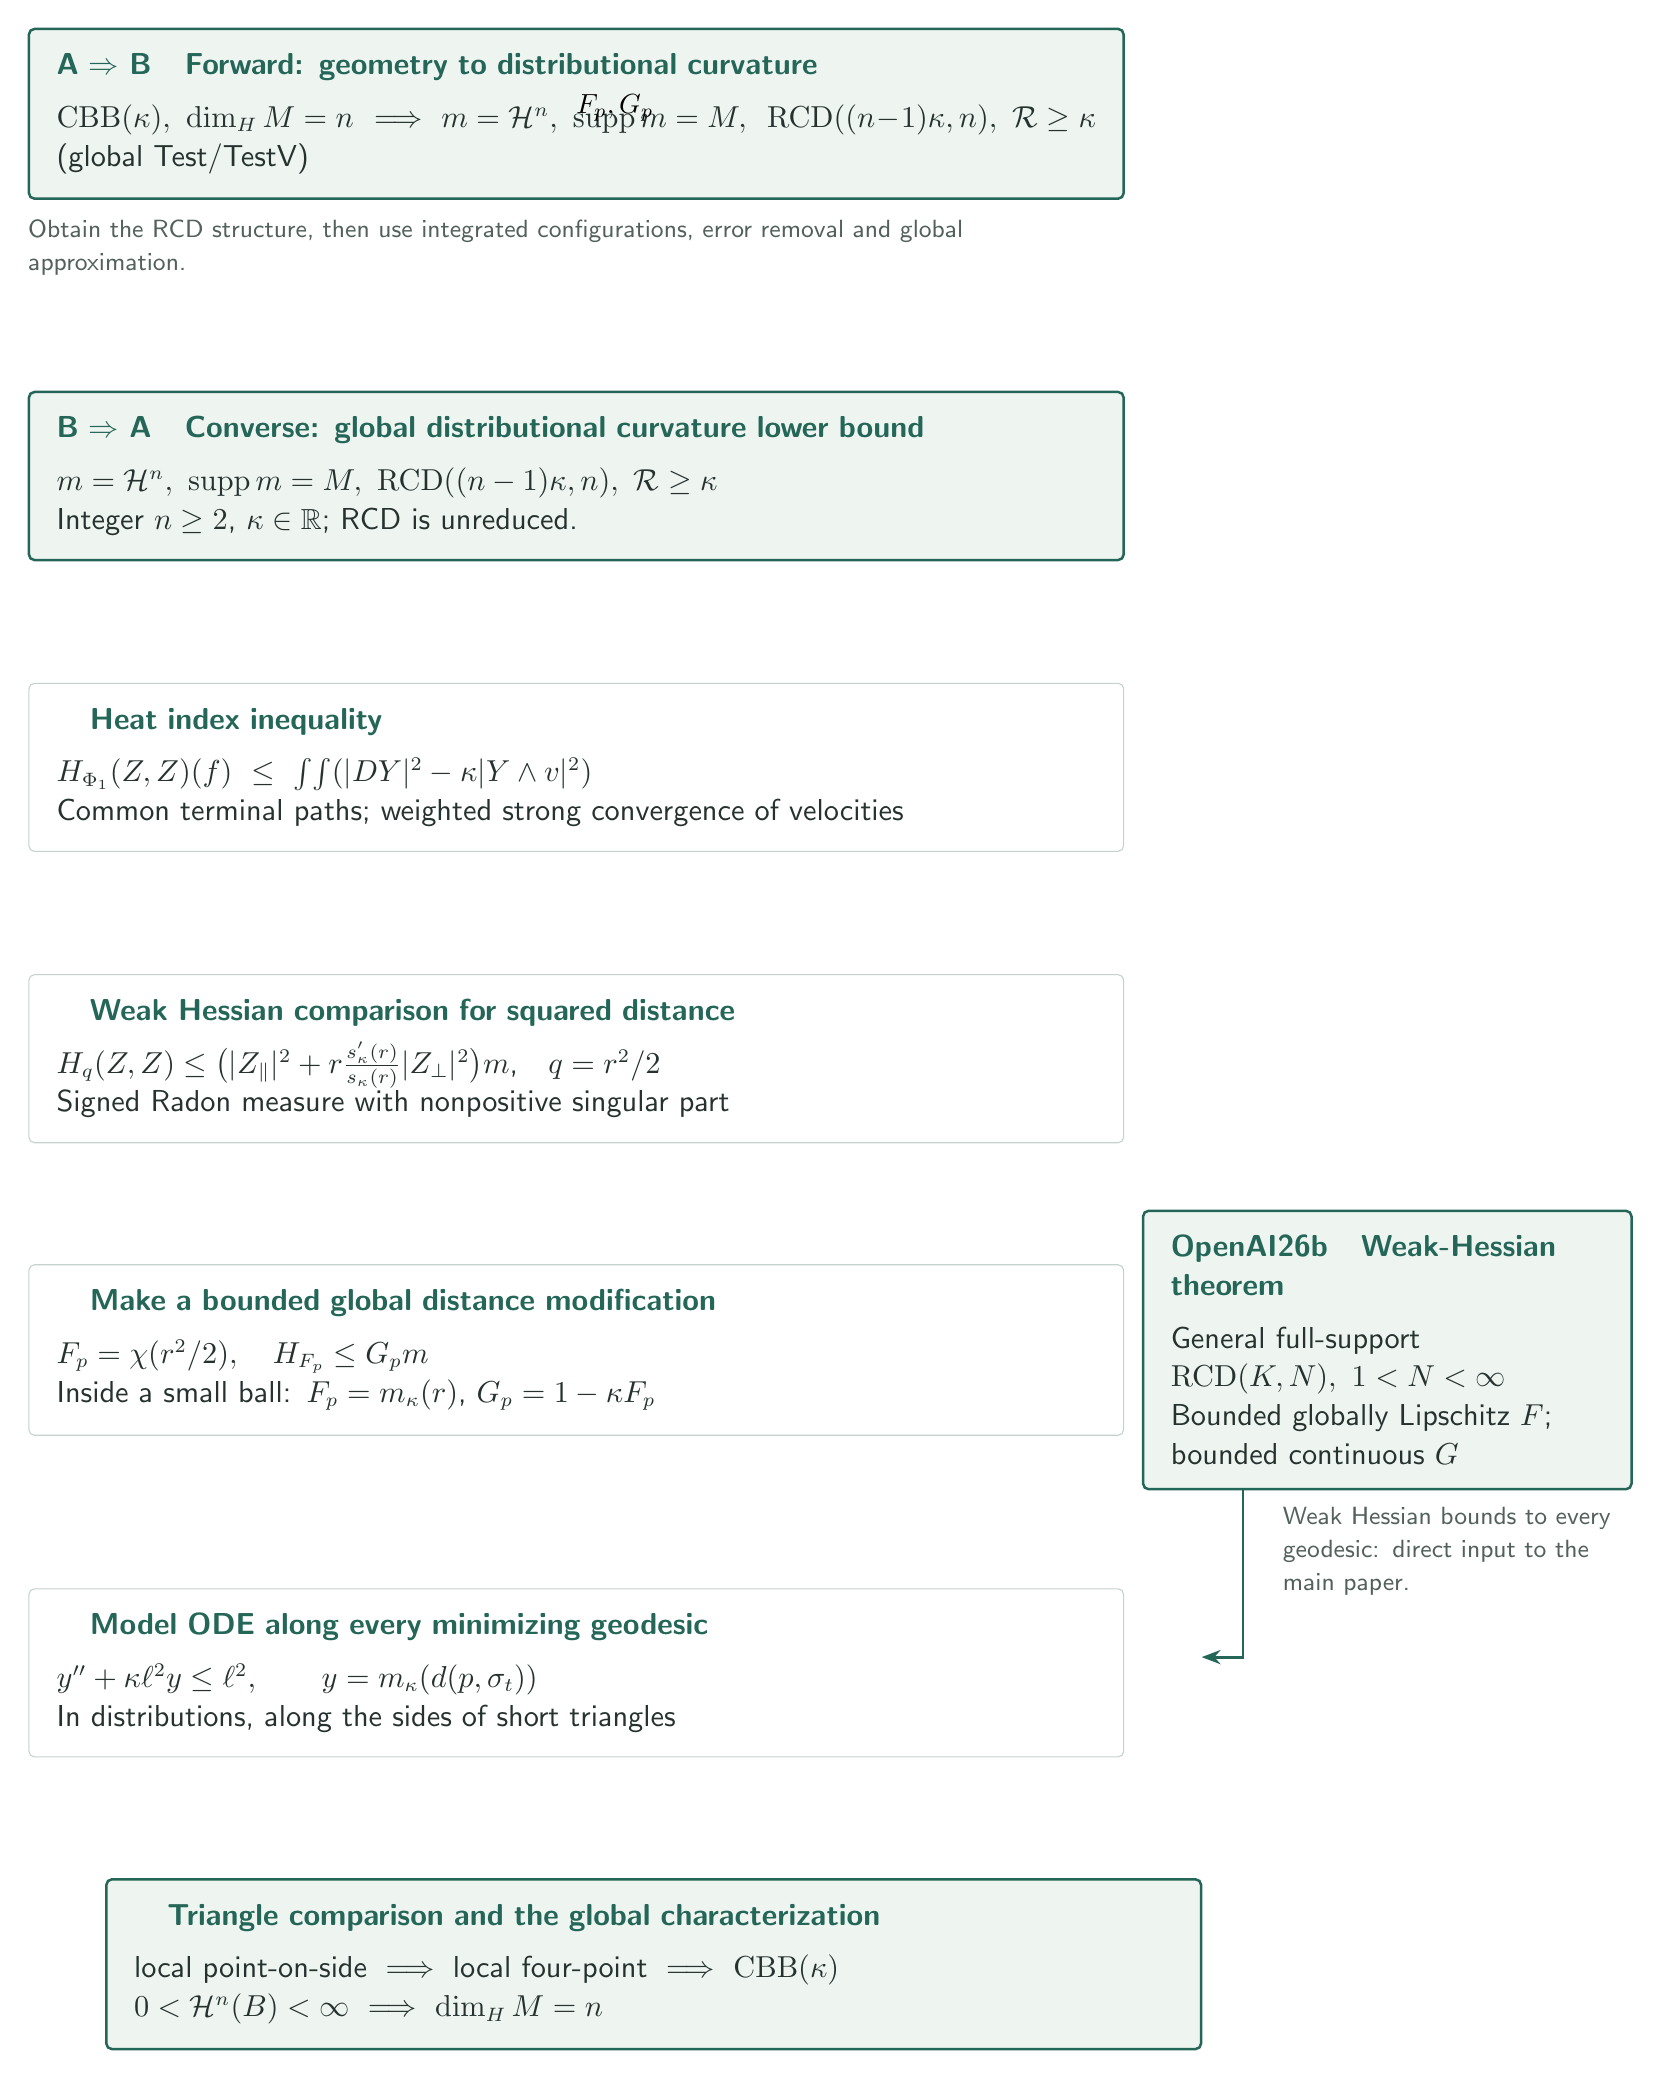
\begin{tikzpicture}

\node[result] (forward) at (0,0) {
\heading{A $\Rightarrow$ B}{順向き：幾何から分布曲率へ}{Forward: geometry to distributional curvature}
$\mathrm{CBB}(\kappa),\ \dim_H M=n$
$\ \Longrightarrow\ m=\mathcal H^n,\ \operatorname{supp}m=M,$
$\ \mathrm{RCD}((n-1)\kappa,n),\ \mathcal R\ge\kappa$\quad
\Tx{（大域Test/TestV）}{(global Test/TestV)}
};
\node[reason,anchor=north west] at ($(forward.south west)+(0,-.25)$) {
\Tx{RCD構造を得て、積分配置・誤差除去・大域近似を行う。}{Obtain the RCD structure, then use integrated configurations, error removal and global approximation.}\\[3pt]
\Cite{forward}
};
\node[result] (input) at (0,-4.6) {
\heading{B $\Rightarrow$ A}{逆向き：大域の分布曲率下界}{Converse: global distributional curvature lower bound}
$m=\mathcal H^n,\ \operatorname{supp}m=M,\ \mathrm{RCD}((n-1)\kappa,n),\ \mathcal R\ge\kappa$\\
\Tx{整数$n\ge2$、$\kappa\in\mathbb R$。RCDはunreduced。}{Integer $n\ge2$, $\kappa\in\mathbb R$; RCD is unreduced.}
};
\node[card] (index) at (0,-8.3) {
\heading{}{熱index不等式}{Heat index inequality}
$H_{\Phi_1}(Z,Z)(f)\ \le\ \int\!\int (|DY|^2-\kappa|Y\wedge v|^2)$\\
\Tx{終点に依存する共通経路、速度の重み付き強収束}{Common terminal paths; weighted strong convergence of velocities}
};
\flow{input}{index}{\Tx{曲率をRiccati恒等式へ入れ、粘性を消す。}{Insert curvature into the Riccati identity and remove viscosity.}\\[3pt]\Cite{index}};
\node[card] (hessian) at (0,-12) {
\heading{}{距離二乗の弱Hessian比較}{Weak Hessian comparison for squared distance}
$H_q(Z,Z)\le\bigl(|Z_\parallel|^2+r\tfrac{s_\kappa'(r)}{s_\kappa(r)}|Z_\perp|^2\bigr)m$,\quad $q=r^2/2$\\
\Tx{符号付きRadon測度、特異部分は非正}{Signed Radon measure with nonpositive singular part}
};
\flow{index}{hessian}{\Tx{非崩壊frame・可算trialでJacobi energyの上界を取る。}{Use noncollapsed frames and countable trials to bound Jacobi energy.}\\[3pt]\Cite{hessian}};
\node[card] (bounded) at (0,-15.7) {
\heading{}{距離を有界大域関数へ修正}{Make a bounded global distance modification}
$F_p=\chi(r^2/2),\quad H_{F_p}\le G_p m$\\
\Tx{内側で$F_p=m_\kappa(r)$、$G_p=1-\kappa F_p$}{Inside a small ball: $F_p=m_\kappa(r)$, $G_p=1-\kappa F_p$}
};
\flow{hessian}{bounded}{\Tx{単調cutoffにより特異部分と半径方向の符号を保つ。}{A monotone cutoff preserves the signs of the singular and radial terms.}\\[3pt]\Cite{modification}};
\node[small,draw=green,fill=tint,line width=.9pt] (companion) at (10.3,-15.7) {
\heading{OpenAI26b}{弱Hessian定理}{Weak-Hessian theorem}
\Tx{一般のfull-support}{General full-support}\\
$\mathrm{RCD}(K,N),\ 1<N<\infty$\\
\Tx{有界大域Lipschitz $F$、有界連続 $G$}{Bounded globally Lipschitz $F$; bounded continuous $G$}\\[3pt]
\Cite{companion}
};
\node[card] (ode) at (0,-19.8) {
\heading{}{すべての最短測地線上のモデルODE}{Model ODE along every minimizing geodesic}
$y''+\kappa\ell^2y\le\ell^2,\qquad y=m_\kappa(d(p,\sigma_t))$\\
\Tx{分布の意味、短い三角形の辺上で成立}{In distributions, along the sides of short triangles}
};
\flow{bounded}{ode}{\Tx{companionを$F_p,G_p$へ適用し、任意測地線へ移す。}{Apply the companion theorem to $F_p,G_p$ to reach every geodesic.}\\[3pt]\Cite{interface}};
\draw[edge] ($(companion.south west)+(.3,0)$) |- ($(ode.east)+(0,.2)$);
\node[reason,text width=4.6cm,anchor=north west] at ($(companion.south west)+(.8,-.2)$) {
\Tx{弱Hessian上界から全測地線へ。主論文への直接入力。}{Weak Hessian bounds to every geodesic: direct input to the main paper.}
};
\node[result] (cbb) at (0,-23.5) {
\heading{}{三角形比較と大域の特徴付け}{Triangle comparison and the global characterization}
$\text{local point-on-side}\ \Longrightarrow\ \text{local four-point}\ \Longrightarrow\ \mathrm{CBB}(\kappa)$\\
$0<\mathcal H^n(B)<\infty\ \Longrightarrow\ \dim_H M=n$
};
\flow{ode}{cbb}{\Tx{1次元比較、局所四点条件、完備length空間で大域化。}{One-dimensional comparison, local four-point criterion, and globalization for a complete length space.}\\[3pt]\Cite{comparison}};

\end{tikzpicture}
\end{document}
